\section{peo\-Transform$<$ EOT $>$ Class Template Reference}
\label{classpeo_transform}\index{peoTransform@{peoTransform}}
The {\bf peo\-Transform}{\rm (p.\,\pageref{classpeo_transform})} class acts only as an interface for creating transform operators - for an example please refer to the {\bf {\bf peo\-Seq\-Transform}{\rm (p.\,\pageref{classpeo_seq_transform})}} and the {\bf {\bf peo\-Para\-SGATransform}{\rm (p.\,\pageref{classpeo_para_s_g_a_transform})}} classes.  


{\tt \#include $<$peo\-Transform.h$>$}

Inheritance diagram for peo\-Transform$<$ EOT $>$::\begin{figure}[H]
\begin{center}
\leavevmode
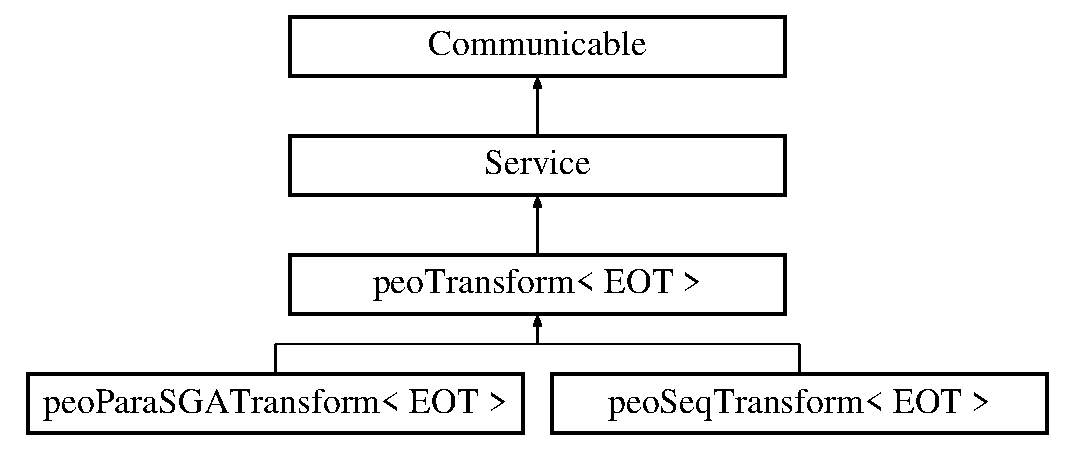
\includegraphics[height=4cm]{classpeo_transform}
\end{center}
\end{figure}


\subsection{Detailed Description}
\subsubsection*{template$<$class EOT$>$ class peo\-Transform$<$ EOT $>$}

The {\bf peo\-Transform}{\rm (p.\,\pageref{classpeo_transform})} class acts only as an interface for creating transform operators - for an example please refer to the {\bf {\bf peo\-Seq\-Transform}{\rm (p.\,\pageref{classpeo_seq_transform})}} and the {\bf {\bf peo\-Para\-SGATransform}{\rm (p.\,\pageref{classpeo_para_s_g_a_transform})}} classes. 



Definition at line 35 of file peo\-Transform.h.

The documentation for this class was generated from the following file:\begin{CompactItemize}
\item 
peo\-Transform.h\end{CompactItemize}
